\section{Background and Motivation}

\emph{Wireless sensor network} (WSN)~\cite{wsn_survey} is a network of spatially dispersed and dedicated sensors that monitor and record the 
physical conditions of the environment and forward the collected data to a central location ~\cite{wsn_wiki} via wireless communication.
WSN can measure environmental conditions such as temperature, sound, humidity, wind, light, wireless channel state information and radio spectrum, etc.
A sensor network becomes a \emph{quantum sensor network} (QSN) when the sensors leverage quantum objects and quantum properties~\cite{RevModPhys.quantumsensing}
such as quantum coherence and quantum entanglement.
Quantum sensors are extremely sensitive to physical quantities such as magnetic field, electric field, quadrature displacement
and phase shift in the optic field.

\para{Classical sensors}. WSNs have various applications~\cite{tsn17-water,sensys10-health,mobicom03-sensor}.
In this thesis, the application we focus on is spectrum surveillance and monitoring~\cite{arani2018} for security and threat detection.
The \emph{core problem} involved in this application is \emph{transmitter localization}~\cite{ton-sensorselect,caitao2023qsn},
 and in particular, \emph{multiple transmitter localization} (\mtl) as 
the number of transmitter present in an area could be more than one and localizing multiple transmitters are not independent.
The reason for being not independent is that a sensor receives an aggregated power from multiple transmitters and separating 
the power from different multiple sources is impractical.
That an aggregated received power is not able to separate is a big challenge for \mtl.

Furthermore, in a shared spectrum paradigm, the presence of an evolving set of authorized users 
(e.g., primary and secondary users) adds to the challenge.
The RF spectrum is a natural resource in great demand due to the unabated increase in mobile (and hence, wireless) data consumption~\cite{Jeffrey14}. 
The research community has addressed this capacity crunch via the development of shared spectrum paradigms, wherein the spectrum 
is made available to unlicensed users (secondaries) as long as they do not interfere with the transmission of licensed incumbents (primaries).
The fundamental objective behind such shared spectrum paradigms is to maximize spectrum utilization,
the viability of such systems depends on the ability to effectively guard the shared spectrum against unauthorized usage. 
The current mechanisms however to locate such unauthorized users (intruders) are human-intensive and time-consuming, 
involving the FCC enforcement bureau which detects violations via complaints and manual investigation~\cite{mobicom17-splot}. 

\begin{figure}[t]
      \centering
      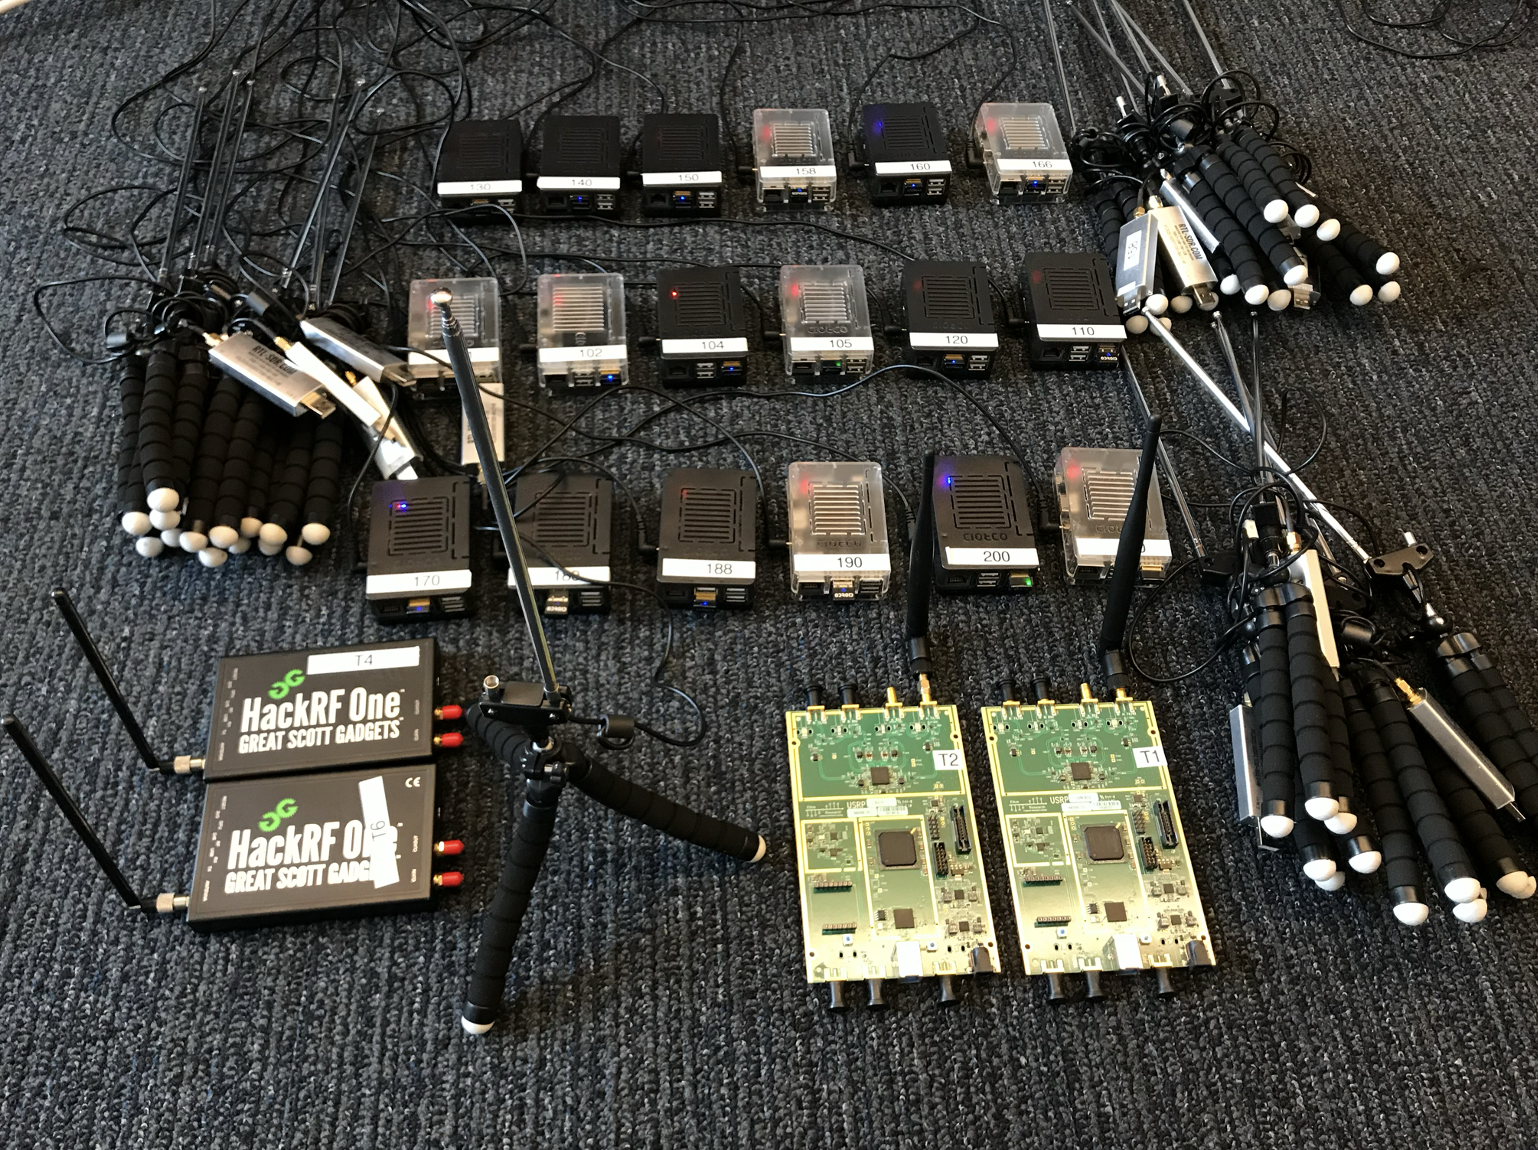
\includegraphics[width=0.6\textwidth]{chapters/introduction/figures/SDR.png}
      \caption{Classical sensors. Radiofrequency sensors used in this thesis. Details see~\S\ref{sec:testbed}} 
      \label{fig:intro-sdr}
\end{figure}

Motivated by the above, we seek an effective technique that can accurately localize multiple simultaneous
intruders and even in the presence of a dynamically changing set of authorized users.
Our solution assumes a network of crowdsourced sensors wherein relatively low-cost spectrum sensors (Fig.~\ref{fig:intro-sdr}) are available
for gathering signal strength in the form of received power.
We introduce two different approaches to the \mtl problem.
The first approach is a hypothesis-driven Bayesian approach, viz. maximum a posterior approach, where wherein each hypothesis is a configuration
(i.e. a combination of $\langle$location, power$\rangle$ pair of the potential intruders), and the goal is to determine the hypothesis 
that best explains the sensor observations.
The second approach is a deep learning-based approach. First, we encode the sensors' observation data into an image.
Then, we frame \mtl as a sequence of two steps: image-to-image translation 
and object detection, each of which is solved using a trained CNN model. 
The first step of image-to-image translation maps an input image representing sensor readings to an image
representing the distribution of transmitter locations, and the second object detection step derives precise locations of
transmitters from the image of transmitter distributions. 
Besides the location, the transmission power is another property of a transmitter that we wish to estimate.
We introduce some novel methods to estimate the power of multiple transmitters.
We also introduce a novel interpolation method for received signal strength.

\para{Quantum sensors.}
We continue the research in transmitter localization, but with the usage of a new kind of sensor -- quantum sensors.
Although classical sensors are omnipresent and work well in general, there are big motivations to explore quantum sensors.
Quantum sensing is an emerging field that leverages quantum objects and properties at atomic/subatomic scales and has 
the potential to sense physical parameters at an unprecedented level of precision.
Therefore, quantum sensing brings new opportunities to new and well-established problems.
For example, physicists in the year 2016 used squeezed state of light to improve the sensitivity of the Laser Interferometer 
Gravitational-wave Observatory (LIGO) detector~\cite{ligo_2015} and successfully detected gravitational waves.
In~\cite{PRL20-qsn}, researchers use some distributed quantum RF-photonic sensors to estimate the amplitude and phase of a radio signal.
They showed the performance of sensing a global property of the RF wave is enhanced (beating the standard quantum limit by over 3 dB)
by leveraging multipartite entangled state and squeezed light.


\begin{figure}[t]
      \centering
      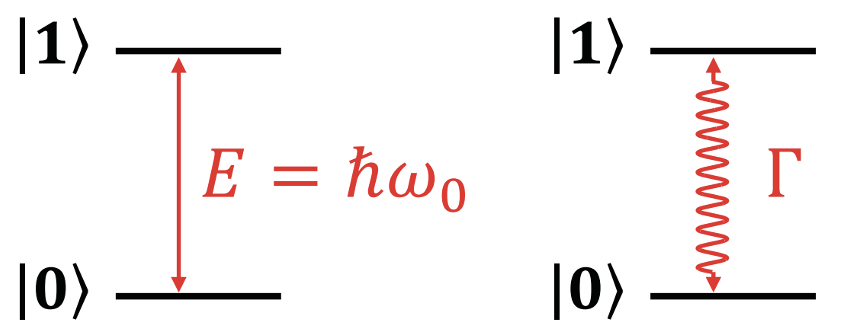
\includegraphics[width=0.45\textwidth]{chapters/introduction/figures/qsensor.png}
      \caption{Quantum sensor theory. Basic features of a two-state quantum sensor, figure from~\cite{RevModPhys.quantumsensing}.
               $\ket{0}$ is the lower energy state and $\ket{1}$ is the higher energy state. Quantum sensing leverages changes in the
               transition frequency $\omega_{0}$ (shifts of the energy level) or the transition rate (transition between energy levels) 
               in response to an external signal $V$.} 
      \label{fig:intro-qsensor}
\end{figure}

\begin{figure}[t]
      \centering
      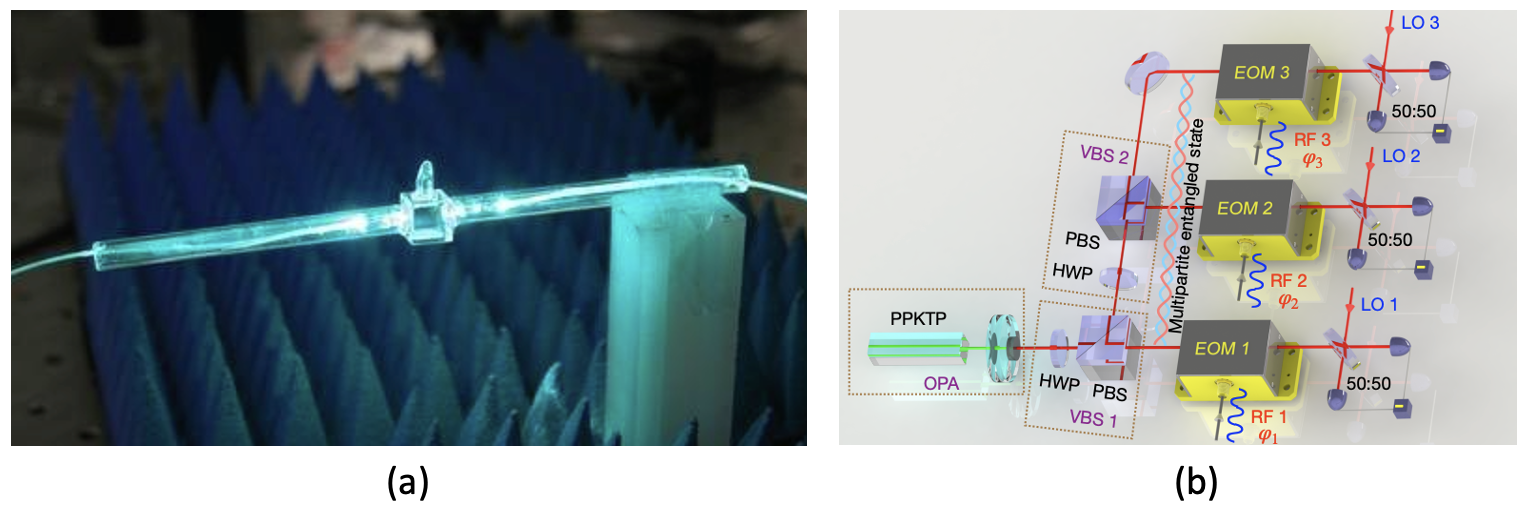
\includegraphics[width=0.85\textwidth]{chapters/introduction/figures/qsensor2.png}
      \caption{Quantum sensors. (a) Fiber-coupled vapor cell for Electric field measurements using Rydberg atoms, figure from~\cite{rydberg};
               (b) Reconfigurable entangled radio frequency photonic sensor network, figure from~\cite{PRL20-qsn}.} 
      \label{fig:intro-qsensor2}
\end{figure}

% Motivated by the above, we aim to leverage quantum sensors to perform some canonical tasks and thus open a new avenue of research.
% The canonical task we picked is RF transmitter localization~\cite{nsdi13-arraytrack,pmc22-deepmtlpro}.
% We consider a network of quantum sensors distributed in a geographic area and a single transmitter active in the area to be localized.
% We pose the localization problem as a quantum state discrimination problem~\cite{bergou-review-2007}. 
% In our approach, the quantum sensor network reports a quantum state, and we discriminate the quantum state via 
% positive-operator valued measure (POVM) and the POVM's output indicates the transmitter location.
% The key challenge here is the scalability challenge, i.e., the method's time and space complexity grows exponentially against the
% number of sensors and the method's localization accuracy decrease against the number of discrete locations.
% To solve the challenge, we propose a two-level POVM method that is comprised of a coarse-level POVM and a fine-level POVM.
% The two level idea is effective and can be generalized into three levels and more.

Our key idea is to pose the transmitter localization problem as a well-studied \emph{quantum state discrimination} (QSD)~\cite{bergou2004,bergou-review-2007,Bae_2015}, 
which allows us to develop viable transmitter localization schemes using quantum sensors. 
We design two high-level schemes to localize a transmitter in a given area deployed with a quantum sensor network.
The first scheme is based on solving an appropriate quantum state discrimination problem using a global measurement, 
while the second scheme uses a trained hybrid quantum-classical circuit to process the quantum sensor data. 
Within the above high-level schemes, we also introduce a two-level localization scheme to improve the performance of the basic one-level schemes.
To evaluate our schemes, we model how a quantum sensor's state evolves due to RF signals from a transmitter at a certain distance. 
Using this model, we evaluate our localization schemes and demonstrate their effectiveness in our custom-built simulator.

Finally, we investigate two problems that are unique in quantum sensor networks. 
The first problem is \emph{optimizing the initial state} of detector sensors 
in quantum sensor networks. We consider a network of quantum sensors, where each sensor is a qubit detector that “fires”, 
i.e., its state changes when an event occurs close by. The change in state due to the firing of a detector is given 
by a unitary operator. The determination of the firing sensor can be posed as a QSD problem which incurs a probability 
of error depending on the initial state and the measurement operator used. We address the problem of determining 
the optimal initial state of the quantum sensor network that incurs a minimum probability of error in determining the firing sensor.
The optimal initial state could be an entangled state.
Thus, the second problem we look into is the \emph{generation and distribution of entangled states}.
Quantum entanglement -- correlation between multiple particles -- is a phenomenon that has no counterpart in the classical world.
It is the physical phenomenon that occurs when a group of particles (electrons, photons, etc) are generated or 
interact in a way such that the quantum state of each particle of the group cannot be described independently 
of the state of the others, including when the particles are separated by a large distance.
In our context of QSNs, entanglement can serve as a resource to enhance the performance of the QSN.
Thus, there is a demand to generate and distribute the entangled state to a network of sensors. 
This a challenging problem in the field of quantum communication.
Physical transmission of quantum states across nodes can incur irreparable communication errors, as the no-cloning theorem proscribes
making independent copies of arbitrary qubits.
The establish of entanglement over long distances is challenging due to the low probability of success of the underlying physical process
(short-distance entanglement and swapping). 
We propose an efficient heuristic approach that efficiently generates an entanglement pair in a quantum network.


\section{Thesis Statement}

This thesis strives to:
\begin{itemize}
      \item Develop novel methods to \emph{localize transmitter(s)} efficiently and accurately using classical and quantum sensor networks.
      \item \emph{Optimize} and \emph{generate} the \emph{initial state} for quantum sensor networks.
\end{itemize}

\section{Thesis Organization}

Towards the thesis statement, we make the following contributions:

\begin{itemize}
    \item In Chapter~\ref{chap:ipsn}, we introduce an efficient hypothesis-based Bayesian approach \ouralgo for multiple transmitter localization (\mtl) problem (\S\ref{sec:time}); 
          A closed-form equation for the estimation of transmission power (\S\ref{sec:ipsn-power});
          A novel received signal strength interpolation method inspired by the power law distribution (\S\ref{sec:inter});
          Extend \ouralgo to accommodate the presence of authorized users (\S\ref{sec:auth}).
    
    \item In Capter~\ref{chap:wowmom-pmc}, we introduce a deep learning-based approach \our for the \mtl problem (\S\ref{sec:translate}, \S\ref{sec:detect});
          Extend \our via deep learning models to accommodate the presence of authorized users (\S\ref{sec:authorized});
          A deep learning-based approach that estimates the transmission power of multiple transmitters (\S\ref{sec:power}).
    
    \item In Chapter~\ref{chap:qce}, we introduce the concept of quantum sensor networks and the model of a quantum sensor (\S\ref{sec:quantum_problem});
          In the context of quantum sensor networks, we pose a transmitter localization problem as a quantum state discrimination problem 
          and introduce a novel quantum localization method \povm and \povmpro based on positive-operator valued measure (\S\ref{sec:povm}).
    
    \item In Chapter~\ref{chap:tqc}, we consider a network of quantum sensors, where each sensor is a qubit detector that "fires", its state changes when an event occurs close by.
          We address the problem of determining the optimal initial global state of a network of quantum sensors that incur a minimum probability of error in determining the firing sensor (\S\ref{sec:tqc_problem}).
          We have proposed both theoretical analytical results (\S\ref{sec:n-ortho}, \S\ref{sec:optimal}) and numerical simulation results(\S\ref{sec:searching}).
          
    \item In Chapter~\ref{chap:swappingtrees}, we introduce an efficient heuristic algorithm \dpalt for routing an entanglement pair.
          The algorithm is Dijkstra-based, and the path selection metric is a closed-form expression that models a path as a tree near accurately (\S\ref{sec:swapping_efficient}).
\end{itemize}


